%% ===========================================================================
%%  Journal of Air Transport Management -- VSI: Green ATM: Tech to Socio-Econ
%%
%%  Every number in this file is a macro from generated/numbers.tex or a table
%%  body from generated/*.tex, written by scripts/run_all.py. Do not type numbers
%%  into the text: change config/parameters.yaml and re-run the pipeline.
%%
%%  Compile: pdfLaTeX -> BibTeX -> pdfLaTeX -> pdfLaTeX (latexmk -pdf main.tex)
%% ===========================================================================

\documentclass[preprint, 12pt, authoryear]{elsarticle}

%% ANONYMISATION SWITCH: \anontrue for the review PDF, \anonfalse otherwise.
\newif\ifanon
\anonfalse

\usepackage{amsmath,amssymb}
\usepackage{graphicx}
\usepackage{booktabs}
\usepackage{longtable}
\usepackage{array}
\usepackage[table]{xcolor}
\usepackage{lineno}
\usepackage{url}
\usepackage{hyperref}
\hypersetup{colorlinks=true, allcolors=blue!50!black}
\raggedbottom

\newenvironment{highlights}
  {\vspace{1em}\noindent\textbf{Highlights}
   \begin{itemize}\setlength{\itemsep}{2pt}\setlength{\parskip}{0pt}}
  {\end{itemize}\vspace{0.5em}}

% Generated by scripts/run_all.py -- do not edit by hand.
\newcommand{\DataLabel}{synthetic}
\newcommand{\NFlights}{60{,}000}
\newcommand{\LnGapLong}{3.98}
\newcommand{\LnGapMedium}{1.98}
\newcommand{\LnGapShort}{1.03}
\newcommand{\PerFlightRatioLong}{52}
\newcommand{\EuroRatioLong}{51}
\newcommand{\EuroLnGapLong}{3.92}
\newcommand{\CalMaxResid}{4.7}
\newcommand{\ScaleRG}{1.01}
\newcommand{\ScaleWB}{1.14}
\newcommand{\OtherEnroute}{6.7}
\newcommand{\SeatKmLong}{41.2}
\newcommand{\SeatShareLong}{10.4}
\newcommand{\RpkBandOne}{131}
\newcommand{\AskBandOne}{107}
\newcommand{\AtmBandOne}{12.0}
\newcommand{\CoShareBandOne}{3.8}
\newcommand{\FlShareBandOne}{23.9}
\newcommand{\RpkBandTwo}{88}
\newcommand{\AskBandTwo}{72}
\newcommand{\AtmBandTwo}{10.3}
\newcommand{\CoShareBandTwo}{20.2}
\newcommand{\FlShareBandTwo}{46.2}
\newcommand{\RpkBandThree}{80}
\newcommand{\AskBandThree}{66}
\newcommand{\AtmBandThree}{7.7}
\newcommand{\CoShareBandThree}{28.3}
\newcommand{\FlShareBandThree}{24.1}
\newcommand{\RpkBandFour}{112}
\newcommand{\AskBandFour}{92}
\newcommand{\AtmBandFour}{2.7}
\newcommand{\CoShareBandFour}{47.7}
\newcommand{\FlShareBandFour}{5.7}
\newcommand{\GammaOne}{0.95}
\newcommand{\GammaSeOne}{0.01}
\newcommand{\GammaTwo}{1.12}
\newcommand{\GammaSeTwo}{0.00}
\newcommand{\GammaThree}{1.18}
\newcommand{\GammaSeThree}{0.01}
\newcommand{\GammaFour}{1.66}
\newcommand{\GammaSeFour}{0.02}
\newcommand{\WaldF}{1477}
\newcommand{\EtaRpk}{-1.10}
\newcommand{\EtaFlight}{0.15}
\newcommand{\AbsAgeRatio}{94}
\newcommand{\EBaseWtw}{245}
\newcommand{\CoTwoBase}{202.7}
\newcommand{\IdxZero}{115}
\newcommand{\IdxThirtyZero}{102}
\newcommand{\CumZero}{6.77}
\newcommand{\IdxOne}{111}
\newcommand{\IdxThirtyOne}{101}
\newcommand{\CumOne}{6.60}
\newcommand{\IdxTwo}{49}
\newcommand{\IdxThirtyTwo}{97}
\newcommand{\CumTwo}{5.42}
\newcommand{\IdxThree}{48}
\newcommand{\IdxThirtyThree}{96}
\newcommand{\CumThree}{5.36}
\newcommand{\ActivityFactor}{1.51}
\newcommand{\RefTtwTwentyFifty}{232}
\newcommand{\RefTtwNoTech}{267}
\newcommand{\PhiTwentyFifty}{0.76}
\newcommand{\ShRenewal}{1.3}
\newcommand{\ShPctRenewal}{1}
\newcommand{\ShCumRenewal}{0.03}
\newcommand{\ShCumPctRenewal}{2}
\newcommand{\ShAtm}{5.9}
\newcommand{\ShPctAtm}{4}
\newcommand{\ShCumAtm}{0.15}
\newcommand{\ShCumPctAtm}{10}
\newcommand{\ShSaf}{151.5}
\newcommand{\ShPctSaf}{92}
\newcommand{\ShCumSaf}{1.18}
\newcommand{\ShCumPctSaf}{84}
\newcommand{\ShZep}{5.4}
\newcommand{\ShPctZep}{3}
\newcommand{\ShCumZep}{0.05}
\newcommand{\ShCumPctZep}{3}
\newcommand{\ShTotal}{164}
\newcommand{\ShCumTotal}{1.41}
\newcommand{\ShSafLongPct}{49}
\newcommand{\ShZepShortPct}{100}
\newcommand{\DelayEndTwo}{52}
\newcommand{\DelayCumTwo}{2.7}
\newcommand{\RstarTwoFive}{0.96}
\newcommand{\RstarTwoTen}{0.92}
\newcommand{\RstarTwoTwenty}{0.84}
\newcommand{\DelayEndThree}{52}
\newcommand{\DelayCumThree}{2.6}
\newcommand{\RstarThreeFive}{0.96}
\newcommand{\RstarThreeTen}{0.92}
\newcommand{\RstarThreeTwenty}{0.84}
\newcommand{\RstarExtTwo}{0.92}
\newcommand{\RstarExtThree}{0.89}
\newcommand{\CumExcessTwoRefR}{4.5}
\newcommand{\CumExcessTwoRefRDelay}{9.0}
\newcommand{\EndExcessTwoRefRDelay}{67}
\newcommand{\MacRenewalLong}{10}
\newcommand{\MacRenewalShortMin}{261}
\newcommand{\MacRenewalShortMax}{272}
\newcommand{\MacAtm}{-68}
\newcommand{\MacBio}{469}
\newcommand{\MacPtl}{2132}
\newcommand{\AtmBreakeven}{245}
\newcommand{\AbatePerAcLong}{55}
\newcommand{\AbatePerAcMedium}{9.5}
\newcommand{\AbatePerAcShort}{5.0}
\newcommand{\CorrNoDelayCumCost}{-7.1}
\newcommand{\CorrNoDelayCumSaving}{7.1}
\newcommand{\CorrNoDelayCumLong}{297}
\newcommand{\CorrNoDelayCost}{17.2}
\newcommand{\CorrNoDelayGap}{217}
\newcommand{\CorrNoDelayLong}{305}
\newcommand{\CorrNoDelayResEnd}{3}
\newcommand{\CorrDelayCost}{77}
\newcommand{\CorrDelayGap}{473}
\newcommand{\CorrDelayResEnd}{66}
\newcommand{\CorrDelayAltSaf}{17}
\newcommand{\CorrDelayCumCost}{71}
\newcommand{\CorrThreeNoDelayResEnd}{50}
\newcommand{\CorrThreeNoDelayCumCost}{34.8}
\newcommand{\AltShareThreeMin}{40}
\newcommand{\AltShareThreeMax}{59}
\newcommand{\ResCumThreeMax}{40}
\newcommand{\SingleATMCovered}{55}
\newcommand{\SingleRenewalCovered}{100}
\newcommand{\SingleAltSafCovered}{100}
\newcommand{\SensRef}{18.8}
\newcommand{\SensMaxSpread}{32}

\newcommand{\EUR}[1]{EUR~#1}

\journal{Journal of Air Transport Management}
\linenumbers

\begin{document}

\begin{frontmatter}

\title{Absorbing sustainable aviation fuel shortfalls in European aviation:
a distance-band model of corrective action through air traffic management,
fleet renewal and alternative supply}

\ifanon
  \author{}
  \address{}
\else
  \author[uhh]{Fabricio Niebles-Atencio\corref{cor1}}
  \ead{fabricio.niebles.atencio@uni-hamburg.de}
  \author[utec]{Luc\'{i}a Rivera-Char\'{u}n}
  \ead{mriverac@utec.edu.pe}
  \cortext[cor1]{Corresponding author.}
  \address[uhh]{Institute of Information Systems, Hamburg Business School,
    University of Hamburg, Von-Melle-Park 5, 20146 Hamburg, Germany}
  \address[utec]{Departamento de Ingenier\'ia Civil y Ambiental, Universidad de
    Ingenier\'ia y Tecnolog\'ia, Jr.\ Medrano Silva 165, Barranco, 15063 Lima, Peru}
\fi

\begin{abstract}
The ReFuelEU Aviation regulation obliges fuel suppliers to deliver rising
minimum shares of sustainable aviation fuel (SAF), but announced production
capacity has repeatedly failed to materialise on time. We ask how much SAF
shortfall European decarbonisation pathways can absorb and which corrective
action restores them at least cost. A well-to-wake model disaggregated into four
flight-distance bands represents air traffic management (ATM) inefficiency,
fleet vintage, SAF supply and zero-emission propulsion with band-specific
feasibility limits. The base-year flight population is generated by
a physically based fuel model calibrated to EUROCONTROL flight and emission
shares and checked against independent data. The SAF mandate delivers \ShPctSaf\% of the 2050 reduction relative to a
no-new-measures reference; zero-emission propulsion contributes \ShPctZep\%. Because the mandate rises in steps, a one-year delay of SAF supply
raises 2050 emissions by \DelayEndTwo\% but cumulative 2025--2050 emissions by
only \DelayCumTwo\%, so terminal-year targets are far more fragile than carbon
budgets. A linear programme combining ATM measures, band-targeted early aircraft
retirement and alternative fuel supply shows that, after an 18\% supply
shortfall, the cumulative budget can be restored at a net saving of
\EUR{\CorrNoDelayCumSaving}\,bn under the assumed prices, through ATM measures
and early retirement of long-haul aircraft; also restoring the 2050 level costs
\EUR{\CorrNoDelayCost}\,bn. With multi-year delays most of the 2050 gap cannot
be closed within delivery-slot and supply limits, and a pathway that already
commits delivery slots to accelerated renewal leaves \CorrThreeNoDelayResEnd\%
of its 2050 gap open even without delay. Implications for SAF target design, ATM regulation and fleet planning follow.
\end{abstract}

\begin{highlights}
\item Well-to-wake distance-band model links SAF supply risk to ATM and fleet levers
\item A one-year SAF delay raises 2050 emissions sharply but cumulative ones only slightly
\item ATM measures are the cheapest corrective lever but close only about half the gap
\item Long-haul early retirement abates most per aircraft and per euro
\item Pathways that pre-commit delivery slots lose corrective headroom
\end{highlights}

\begin{keyword}
Sustainable aviation fuel \sep ReFuelEU Aviation \sep Air traffic management
\sep Fleet renewal \sep Linear programming \sep Decarbonisation pathways
\end{keyword}

\end{frontmatter}


%% ===========================================================================
\section{Introduction}
\label{sec:intro}

European aviation is expected to reduce its emissions while traffic grows by
about 1.6\% per year to 2050 \citep{eurocontrol2024outlook}. The sector's
abatement levers differ in speed, cost and reach. Sustainable aviation fuels
(SAF) can be used by every existing aircraft, which is why the ReFuelEU
Aviation regulation places the largest share of the effort on them: fuel
suppliers at Union airports must supply minimum shares of 2\% in 2025, 6\% in
2030, 20\% in 2035, 34\% in 2040, 42\% in 2045 and 70\% in 2050, with a
synthetic-fuel sub-mandate reaching 35\% \citep{eu2023}. Fleet renewal lowers
fuel burn per kilometre but is bounded by aircraft manufacturing capacity.
Operational efficiency in air traffic management (ATM) is fast to deploy but
small in scale, and zero-emission propulsion is limited by range to short
flights \citep{akinola2025, uddin2025}.

Two features of the problem are poorly represented in existing assessments.
The first is that the levers act unevenly across flight distances. Flights
shorter than 500\,km account for about 24\% of European departures but only
3.8\% of CO$_2$, whereas flights longer than 4000\,km account for 6\% of
departures and 48\% of CO$_2$ \citep{eurocontrol2021}. ATM inefficiency is
concentrated in the terminal phases and is therefore a larger share of fuel on
short flights; zero-emission propulsion is feasible only there; and SAF and
fleet renewal are the only levers that reach the long-haul flights that dominate
the footprint. A model that treats the system as homogeneous cannot represent
these interactions.

The second feature is supply risk. Of the SAF capacity announced for 2024 only
about a quarter was operational on time, and modelled EU shortfalls range from
18--43\% of the 2030 mandate and 5--35\% of the 2050 mandate
\citep{martulli2025}. A mandate expressed as a minimum share is binding on
paper but bounded in practice by the fuel that is available. Robust
decarbonisation strategies under background uncertainty have been studied at
the system level \citep{costaalves2026, dray2022, bergero2023}, and the
cost-effectiveness of mitigation options is commonly assessed with
abatement-cost metrics \citep{schafer2016, salgas2025}. The link between the
observed announcement--realisation gap and the operational and fleet levers
that could compensate for it, distance band by distance band, has not been
quantified.

This paper addresses that link. Its contributions are as follows.
\begin{enumerate}
  \item A well-to-wake (WTW) emissions model disaggregated into four distance
  bands, in which SAF enters as a supply-constrained quantity, fleet intensity
  follows from a vintage model, and ATM inefficiency is derived per flight from
  taxi, arrival-sequencing and en-route components
  (Section~\ref{sec:model}).
  \item A physically based base-year flight population calibrated to
  EUROCONTROL flight and emission shares and validated against independent
  seat-kilometre and per-passenger intensity data (Section~\ref{sec:data}).
  \item A Shapley attribution of each pathway's reduction to levers and bands,
  which separates the contributions of levers that scenarios usually change
  together (Section~\ref{sec:results-paths}).
  \item A stress test of SAF-dependent pathways against supply delays and
  realisation shortfalls, with a closed-form critical realisation rate, and a
  linear programme that returns the minimum-cost corrective portfolio of ATM
  measures, band-targeted early retirement and alternative fuel supply
  (Sections~\ref{sec:results-stress} and~\ref{sec:results-corr}).
\end{enumerate}
We address four research questions. RQ1: How do emissions, intensity and ATM
inefficiency differ across distance bands? RQ2: Which levers deliver the
reductions of each pathway, in which bands? RQ3: How much SAF supply disruption
can each pathway absorb before missing its targets? RQ4: What is the
minimum-cost corrective action, by lever and band, and what remains
uncompensable?

Section~\ref{sec:model} presents the model, Section~\ref{sec:data} the data,
calibration and scenarios, Section~\ref{sec:results} the results, and
Section~\ref{sec:discussion} the economic, management and policy implications
together with the limitations. Section~\ref{sec:conclusions} concludes.

%% ===========================================================================
\section{Model}
\label{sec:model}

\subsection{Well-to-wake emissions by distance band}

Let $d\in\{1,\dots,4\}$ index the distance bands 0--500, 500--1500, 1500--4000
and $>$4000\,km, and $t$ the year, with base year $t_0=2024$. Fuel burned by
conventional aircraft in band $d$ is
\begin{equation}
\label{eq:fuel}
F_{d,t} \;=\; F^{\mathrm{eff}}_{d,t_0}\,\frac{A_{d,t}}{A_{d,t_0}}\;
\Phi_{d,t}\;\bigl(1+a_{d,t}\bigr)\;\bigl(1-\pi_{d,t}\bigr),
\end{equation}
where $F^{\mathrm{eff}}_{d,t_0}$ is base-year fuel net of ATM inefficiency,
$A_{d,t}$ is activity (flights), $\Phi_{d,t}$ is the fleet fuel-intensity index
($\Phi_{d,t_0}=1$), $a_{d,t}$ is the ATM excess-fuel ratio and $\pi_{d,t}$ the
share of flights operated by zero-emission propulsion (ZEP). The fuel-equivalent
of ZEP flights, $R_{d,t}$, is the same expression with $\pi_{d,t}$ in place of
$(1-\pi_{d,t})$. System emissions are
\begin{equation}
\label{eq:emis}
E_t \;=\; e\Bigl(\sum_d F_{d,t} - \theta^{\mathrm{bio}} S^{\mathrm{bio}}_t
- \theta^{\mathrm{syn}} S^{\mathrm{syn}}_t\Bigr) \;+\; e\,\kappa_t\sum_d R_{d,t},
\end{equation}
where $S^{\mathrm{bio}}_t$ and $S^{\mathrm{syn}}_t$ are the quantities of
bio-based and synthetic SAF used, $\theta$ their life-cycle emission reductions
relative to fossil kerosene, and $\kappa_t$ the WTW intensity of the ZEP energy
carrier relative to the kerosene it replaces.

\paragraph{Emission boundary} Equation~\eqref{eq:emis} is a WTW inventory
throughout. The fossil factor is $e = 89\,\mathrm{g\,CO_2e/MJ} \times
43.15\,\mathrm{MJ/kg} \approx 3.84$\,t\,CO$_2$e per tonne of fuel
\citep{icaocorsia}, which adds upstream emissions to the tank-to-wake (TTW)
combustion factor $\varepsilon=3.16$\,t\,CO$_2$/t. Because $\theta$ is a WTW
reduction, it multiplies $e$ and never $\varepsilon$: at the tailpipe a tonne of
SAF emits about as much CO$_2$ as a tonne of kerosene, and its benefit arises
upstream. Applying $\theta$ to $\varepsilon$ would mix a combustion factor with a
life-cycle reduction. The same boundary is applied to ZEP through $\kappa_t$;
setting $\kappa_t=0$ would credit ZEP with a full life-cycle benefit while
crediting SAF only with $\theta<1$. Two consequences follow. Indexed
trajectories are unaffected by the choice between $e$ and $\varepsilon$ in the
fossil term, because a constant factor cancels in a ratio; absolute tonnages are
not. Inventories reported TTW, such as those of EUROCONTROL, are therefore
rescaled by $e/\varepsilon$ when compared with the WTW results. Under the EU
Emissions Trading System convention, eligible SAF carries a zero emission
factor, which corresponds to $\theta=1$ with $\varepsilon$ in place of $e$.

\subsection{Intensity indicators}

Emissions per available seat-kilometre (ASK) describe the fleet; emissions per
revenue passenger-kilometre (RPK) describe how efficiently passengers are
carried:
\begin{equation}
\label{eq:intensity}
\iota^{\mathrm{ASK}}_{d,t} = \frac{E_{d,t}}{A_{d,t}\,\bar L_d\,\bar S_d},
\qquad
\iota^{\mathrm{RPK}}_{d,t} = \frac{E_{d,t}}{A_{d,t}\,\bar L_d\,\bar S_d\,\lambda_{d,t}}
= \frac{\iota^{\mathrm{ASK}}_{d,t}}{\lambda_{d,t}},
\end{equation}
with mean stage length $\bar L_d$, seats $\bar S_d$ and load factor
$\lambda_{d,t}$. Load factor enters only the RPK indicator. At flight level a
higher load factor raises take-off mass and therefore fuel burn slightly, so it
raises emissions per flight while lowering emissions per passenger; both
effects are represented in the flight model (Section~\ref{sec:flightmodel}).

\subsection{SAF mandate and supply}

ReFuelEU sets minimum shares $\sigma^{\min}_t$ and synthetic sub-shares
$\sigma^{\mathrm{syn}}_t$, defined per period and therefore stepwise in time
\citep{eu2023}. The obligation falls on fuel suppliers and, until 2034, may be
met as a volume-weighted average across Union airports. The mandate is a
fleet-wide lower bound; the upper bound is the SAF available, $\bar S_t$:
\begin{equation}
\label{eq:saf}
\sigma^{\min}_t \sum_d F_{d,t} \;\le\; S^{\mathrm{bio}}_t + S^{\mathrm{syn}}_t \;\le\; \bar S_t,
\qquad
S^{\mathrm{syn}}_t \;\ge\; \sigma^{\mathrm{syn}}_t \sum_d F_{d,t}.
\end{equation}
When $\bar S_t$ falls below the mandated quantity, the mandate cannot be met;
this is the case examined in the stress test. Equation~\eqref{eq:emis} implies
that for a given quantity of SAF, system emissions do not depend on how that
quantity is allocated across bands:
\begin{equation}
\label{eq:neutral}
\sum_d E_{d,t} \;=\; e\Bigl(\sum_d F_{d,t} - \theta^{\mathrm{bio}}S^{\mathrm{bio}}_t
- \theta^{\mathrm{syn}}S^{\mathrm{syn}}_t\Bigr) + e\,\kappa_t\sum_d R_{d,t}
\quad\text{for any allocation.}
\end{equation}
In a CO$_2$ model, preferential allocation of SAF to long-haul flights is
therefore abatement-neutral; arguments for it must rest on non-CO$_2$ effects,
which are larger on long cruise segments \citep{voigt2021, lee2021}, or on cost
pass-through. Band-level results below allocate SAF pro rata to fuel. A second
implication matters for corrective action: when supply binds, a tonne of fuel
saved by any other lever displaces fossil kerosene and abates $e$, not
$e(1-\theta\sigma)$.

\subsection{Fleet vintage and aircraft age}
\label{sec:fleet}

Each band's fleet is represented by annual cohorts of age $0,\dots,L-1$ with
$L=25$ years. The fuel-burn multiplier of a cohort of age $a$ relative to a
current-generation aircraft is
\begin{equation}
\label{eq:vintage}
m_{c}(a) \;=\; g_c(a)\,(1+\rho\,a), \qquad
g_c(a) = \begin{cases} 1 & a \le \bar a_c\\ (1-\Delta_c)^{-1} & a>\bar a_c\end{cases},
\end{equation}
for aircraft class $c$ (regional, narrow-body, wide-body), with generation step
$\Delta_c$, current-generation age limit $\bar a_c$ and deterioration $\rho$.
Cohorts retire at age $L$ and are replaced by deliveries whose multiplier falls
by a factor $(1-\tau)$ per year. Accelerated renewal retires the oldest cohorts
early, up to a delivery-slot limit expressed as a share of the band's fleet.
$\Phi_{d,t}$ is the kilometre-weighted mean multiplier divided by its base-year
value.

This structure answers how aircraft age enters the analysis. Because age acts
multiplicatively on fuel burn, the natural regression on flight-level data is
\begin{equation}
\label{eq:reg}
\ln y_i \;=\; \beta_0 + \sum_{d=2}^{4}\beta_d B_{id} + \sum_{d=1}^{4}\gamma_d\,B_{id}A_i
+ \eta\,\Lambda_i + \mathbf{x}_i'\boldsymbol{\zeta} + \epsilon_i,
\end{equation}
with band indicators $B_{id}$, age $A_i$, load factor $\Lambda_i$ and controls
$\mathbf{x}_i$ (log distance, aircraft class). Each $\gamma_d$ is a
semi-elasticity: the \emph{proportional} change in emissions per year of age in
band $d$. The \emph{absolute} change is $\partial E_i/\partial A_i = \gamma_d
E_i$, which grows with the band's emission level even when the $\gamma_d$ are
equal. A common slope $\gamma$ therefore already implies a much larger absolute
age effect at long range; whether the relative effect also differs is tested
by $H_0\!:\gamma_4=\gamma_1$. The load-factor effect is estimated twice, with
$y_i$ equal to emissions per flight and to emissions per RPK.

\subsection{Air traffic management inefficiency}
\label{sec:atm}

ATM-related excess fuel of flight $i$ is the sum of additional taxi-out time,
additional arrival-sequencing (ASMA) time and en-route inefficiency within
European airspace:
\begin{equation}
\label{eq:atm}
x_i \;=\; \tau^{\mathrm{taxi}} q^{\mathrm{taxi}}_{c(i)} \;+\; \tau^{\mathrm{asma}} q^{\mathrm{hold}}_{c(i)}
\;+\; \bigl(k^{\mathrm{KEA}} + k^{\mathrm{oth}}\bigr)\, C_i\,\frac{\min(D_i, D^{\mathrm{EU}})}{D_i},
\end{equation}
where $\tau$ are additional times, $q$ class-specific fuel flows, $k^{\mathrm{KEA}}$
the horizontal en-route flight-efficiency excess, $k^{\mathrm{oth}}$ the
remaining (vertical and other) inefficiency, $C_i$ cruise fuel, $D_i$ stage
length and $D^{\mathrm{EU}}$ the distance flown in European airspace. The two
fixed terminal terms make the relative inefficiency largest on short flights,
and the airspace limit makes it smallest on long-haul flights. The band ratio
$a_{d,t_0}$ in Eq.~\eqref{eq:fuel} is the band's excess divided by its efficient
fuel. ATM measures recover a fraction of this pool that rises linearly to a
ceiling by a target year; the pool cannot be fully recovered, because part of
the inefficiency is needed for separation and weather \citep{prc2021}.

\subsection{Zero-emission propulsion}

Battery-electric and hydrogen aircraft are limited by range
\citep{akinola2025, uddin2025}. Penetration is bounded by band-specific ceilings,
$0\le\pi_{d,t}\le\bar\pi_d$ with $\bar\pi_1>\bar\pi_2>\bar\pi_3=\bar\pi_4=0$,
and ramps up from an entry-into-service year.

\subsection{SAF supply disruption and tolerance}
\label{sec:stressmodel}

Supply disruption is parameterised by a ramp-up delay $\delta$ (years) and a
persistent realisation rate $r\in(0,1]$:
\begin{equation}
\label{eq:disrupt}
S_t(\delta, r) \;=\; r\,\sigma^{\min}_{t-\delta}\, F^{\mathrm{nom}}_t,
\end{equation}
applied separately to the bio and synthetic components, where
$F^{\mathrm{nom}}_t$ is the pathway's nominal fuel demand. A delay shifts the
capacity ramp in time; $r<1$ represents capacity that never materialises. The
evidence in \citet{martulli2025} bounds $r$ to roughly $[0.57, 0.95]$.

For each pathway $p$ we consider two targets: the cumulative 2025--2050 budget
$B_p=\sum_t E^{p,\mathrm{nom}}_t$ and the 2050 level $E^{p,\mathrm{nom}}_{2050}$,
each with an optional slack $s\ge 0$. For a shortfall without delay,
Eq.~\eqref{eq:emis} gives the critical realisation rate for the 2050 target in
closed form:
\begin{equation}
\label{eq:rstar}
r^{*}_p \;=\; \frac{F_{2050} + \kappa_{2050}R_{2050} - \bar E_p/e}
{\theta^{\mathrm{bio}}S^{\mathrm{bio}}_{2050} + \theta^{\mathrm{syn}}S^{\mathrm{syn}}_{2050}},
\end{equation}
with $\bar E_p=(1+s)E^{p,\mathrm{nom}}_{2050}$ for an internal target or a level
common to all pathways for an external one. For internal targets and
$\kappa_{2050}=0$, $r^*_p = 1 - s\,(1/(\bar\theta\sigma^{\min}_{2050})-1)$, so
tolerance depends only on the terminal blend and its life-cycle reduction;
efficiency levers matter for robustness only against external targets.

\subsection{Minimum corrective action}
\label{sec:lpmodel}

When a disruption breaks a target, three levers can compensate. Alternative
SAF $x^{A}_t$ (imports or book-and-claim supply) abates $e\,\theta^{\mathrm{bio}}$
per tonne and is limited to a share of annual fuel demand. Early retirement of
$x^{R}_{d,t}$ aircraft in band $d$ saves $f_{d,t}$ tonnes of fuel per year for
the $R$ years by which retirement is advanced, limited by the delivery slots the
pathway does not already use. Additional ATM measures save $x^{O}_{d,t}$ tonnes
of fuel, limited by the part of the benefit pool between the nominal recovery
and an upper ceiling. With $G_t=E_t(\delta,r)-E^{\mathrm{nom}}_t$ the gap
created by the disruption, the minimum-cost corrective portfolio solves
\begin{align}
\label{eq:lp}
\min\;& \sum_t c^{A}x^{A}_t + \sum_{d,t} C^{R}_{d,t}x^{R}_{d,t} + \sum_{d,t} c^{O}x^{O}_{d,t}
+ M\bigl(u^{\mathrm{cum}}+u^{2050}\bigr)\\
\text{s.t.}\;& \sum_t\Bigl[G_t - e\theta^{\mathrm{bio}}x^{A}_t
- e\sum_d\Bigl(\sum_{\tau=t-R+1}^{t} f_{d,\tau}x^{R}_{d,\tau} + x^{O}_{d,t}\Bigr)\Bigr] \le u^{\mathrm{cum}}, \nonumber\\
& G_{2050} - e\theta^{\mathrm{bio}}x^{A}_{2050}
- e\sum_d\Bigl(\sum_{\tau=2051-R}^{2050} f_{d,\tau}x^{R}_{d,\tau} + x^{O}_{d,2050}\Bigr) \le u^{2050}, \nonumber\\
& 0\le x^{A}_t\le \bar x^{A}_t,\quad 0\le x^{R}_{d,t}\le \bar x^{R}_{d,t},\quad
0\le x^{O}_{d,t}\le \bar x^{O}_{d,t},\quad u\ge 0. \nonumber
\end{align}
Here $c^{A}$ is the SAF price premium over fossil fuel, $C^{R}_{d,t}$ the net cost
of advancing one retirement and $c^{O}$ the net cost per tonne of fuel saved by
ATM measures. The penalty $M$ makes the residuals $u$ positive only when the
levers cannot close the gap within their limits; a positive residual is the part
of the disruption that requires measures outside the model, such as demand
management or carbon removal. Measures with negative net cost would already be adopted in the nominal pathway
unless barriers prevented it, so in the objective their cost is set to zero plus
a small charge per tonne abated (the same for every lever), ordered by their net
cost; they are therefore used only where needed, and their true net cost is
reported. The static abatement cost of advancing one retirement in
band $d$ is
\begin{equation}
\label{eq:mac}
\mu_d \;=\; \frac{\mathrm{CRF}\,\bigl(K_d - V_d\bigr) - P^{\mathrm{fuel}} f_d}{e\,f_d},
\qquad f_d = U_d\,\phi_d\,\bigl(m^{\mathrm{old}}_d - m^{\mathrm{new}}_d\bigr)\bigl(1-\pi_d\bigr),
\end{equation}
with new-aircraft value $K_d$, residual value $V_d$, capital recovery factor
CRF, fuel price $P^{\mathrm{fuel}}$, utilisation $U_d$ (km per year) and fuel
burn per kilometre $\phi_d$ (scaled by the share $1-\pi_d$ of the band still
flown on kerosene), following the abatement-cost logic of
\citet{schafer2016} and \citet{salgas2025}. Abatement per aircraft is
proportional to $f_d$ and favours long-haul aircraft; abatement per euro also
depends on the capital outlay $K_d-V_d$, and the ranking is an empirical result,
not an assumption.

%% ===========================================================================
\section{Data, calibration and scenarios}
\label{sec:data}

\subsection{Flight-level fuel model}
\label{sec:flightmodel}

No open flight-level emission inventory with aircraft age and load factor exists
for Europe. The base-year population is therefore generated from a physically
based fuel model, and every downstream result can be recomputed on observed
flights with the same schema. We sample \NFlights\ flights with the 2019
EUROCONTROL band shares of departures \citep{eurocontrol2021, prc2021}, draw
stage lengths within each band, assign an aircraft class from band-specific
class mixes, and draw age and load factor. Fuel per flight is
\begin{equation}
\label{eq:flightfuel}
F_i \;=\; \bigl[\ell_{c} + \kappa_c\,\phi^{0}_{c}\,D_i\,(1+\omega_c D_i)\bigr]\,
m_{c}(A_i)\,\bigl[1+\psi(\Lambda_i-\bar\Lambda)\bigr] \;+\; x_i,
\end{equation}
with landing-and-take-off fuel $\ell_c$, current-generation cruise fuel per
kilometre $\phi^0_c$, a fuel-weight curvature $\omega_c$, the vintage multiplier
of Eq.~\eqref{eq:vintage}, payload sensitivity $\psi$ and the ATM excess of
Eq.~\eqref{eq:atm}. Band differences therefore arise from distance, aircraft
size and fleet composition rather than from assumed band means.

\subsection{Calibration and validation}

Two class scalings, $\kappa_{\mathrm{RG}}$ and $\kappa_{\mathrm{WB}}$, are fitted
so that band CO$_2$ shares reproduce the EUROCONTROL 2019 shares; the
narrow-body scaling is fixed at one and anchors the level. The remaining
en-route inefficiency $k^{\mathrm{oth}}$ is fitted so that the ATM benefit pool
of flights below 4000\,km equals the 9\% reported by the Performance Review
Commission \citep{prr2024}. The fitted scalings are $\kappa_{\mathrm{RG}}=\ScaleRG$
and $\kappa_{\mathrm{WB}}=\ScaleWB$, close to the engineering start values, and
$k^{\mathrm{oth}}=\OtherEnroute$\%. The largest relative deviation from the
calibration targets is \CalMaxResid\%. The band totals are then scaled to the
\CoTwoBase\,Mt CO$_2$ (TTW) emitted in the EUROCONTROL area in 2024
\citep{prr2024}.

Three checks use data not used in the fit (Table~\ref{tab:cal}). The long-haul
band carries \SeatShareLong\% of seats and \SeatKmLong\% of seat-kilometres,
against 10\% and ``more than 40\%'' reported by \citet{eurocontrol2021}, and
emissions per RPK follow the U-shaped pattern across bands found in independent
German emission factors \citep{ifeu2026}. As a comparison with an external
projection, the reference pathway without any improvement of new deliveries
reaches \RefTtwNoTech\,Mt CO$_2$ (TTW) in 2050, against 271\,Mt in EUROCONTROL's
case without significant measures \citep{eurocontrol2024outlook}; with the
assumed 1\% annual improvement of new deliveries it reaches \RefTtwTwentyFifty\,Mt,
an improvement that the outlook counts among its fleet and technology measures.

\begin{table}[htbp]
\centering
\caption{Calibration and validation of the base-year flight population. Flight
and CO$_2$ shares in \%; intensities in g CO$_2$ (TTW). Targets for flight and
CO$_2$ shares from \citet{eurocontrol2021} and \citet{prc2021}; the
per-RPK ratio is compared with \citet{ifeu2026}, which was not used in the fit.}
\label{tab:cal}
\footnotesize
\setlength{\tabcolsep}{3pt}
\begin{tabular}{lrrrrrrrrr}
\toprule
 & \multicolumn{2}{c}{Flights} & \multicolumn{2}{c}{CO$_2$} & \multicolumn{2}{c}{Intensity} &
 \multicolumn{2}{c}{RPK ratio} & ATM \\
\cmidrule(lr){2-3}\cmidrule(lr){4-5}\cmidrule(lr){6-7}\cmidrule(lr){8-9}
Band & target & model & target & model & /ASK & /RPK & model & ifeu & excess \% \\
\midrule
\csname @@input\endcsname generated/tab_calibration.tex
\bottomrule
\end{tabular}
\end{table}

\subsection{Scenarios}

Four nested pathways are defined by the levers they activate
(Table~\ref{tab:scen}). All share traffic growth of 1.6\% per year
\citep{eurocontrol2024outlook} and natural fleet renewal with a 1\% annual
improvement of new deliveries. S0 is a counterfactual without new measures; it
holds the SAF share at its 2024 level of 0.6\% \citep{easa2025refuel} and is
therefore below the legal mandate. S1 adds ATM measures that recover half of the
benefit pool by 2035. S2 adds the ReFuelEU mandate, fully supplied. S3 adds
zero-emission propulsion from 2035 and accelerated renewal that lowers the
retirement age to 20 years within the delivery-slot limit. All parameters,
their sources and their status (sourced, derived, calibrated, assumed) are
listed in~\ref{app:params}.

\begin{table}[htbp]
\centering
\caption{Scenario definitions. All scenarios include traffic growth and natural
fleet renewal.}
\label{tab:scen}
\small
\setlength{\tabcolsep}{4pt}
\begin{tabular}{llcccc}
\toprule
 & & ATM & SAF & ZEP & Accelerated \\
 & Pathway & measures & mandate & propulsion & renewal \\
\midrule
S0 & Reference & -- & -- & -- & -- \\
S1 & Operational efficiency & \checkmark & -- & -- & -- \\
S2 & SAF mandate & \checkmark & \checkmark & -- & -- \\
S3 & Low-emission propulsion & \checkmark & \checkmark & \checkmark & \checkmark \\
\bottomrule
\end{tabular}
\end{table}

%% ===========================================================================
\section{Results}
\label{sec:results}

\subsection{Band structure and ATM inefficiency}
\label{sec:results-bands}

Figure~\ref{fig:bands} shows where flights, seat-kilometres and emissions sit.
On average a long-haul flight emits about \PerFlightRatioLong\ times as much as a
flight below 500\,km. Most of this difference reflects
distance and aircraft size, not inefficiency. Per seat-kilometre the long-haul
band emits \AskBandFour\,g, against \AskBandTwo\,g and \AskBandThree\,g in the
two medium bands and \AskBandOne\,g below 500\,km, where take-off and landing
dominate. The concentration of emissions in long-haul flying therefore
describes where abatement must reach, not that long-haul flying is
intrinsically wasteful.

ATM inefficiency has the opposite profile. Excess fuel is \AtmBandOne\% of fuel
below 500\,km, \AtmBandTwo\% and \AtmBandThree\% in the medium bands and
\AtmBandFour\% above 4000\,km, because terminal inefficiency is a fixed cost per
flight and only the European part of a long-haul trajectory is affected. ATM
measures are thus a short-haul and medium-haul lever, complementary to fleet
renewal, whose leverage grows with distance.

\begin{figure}[htbp]
\centering
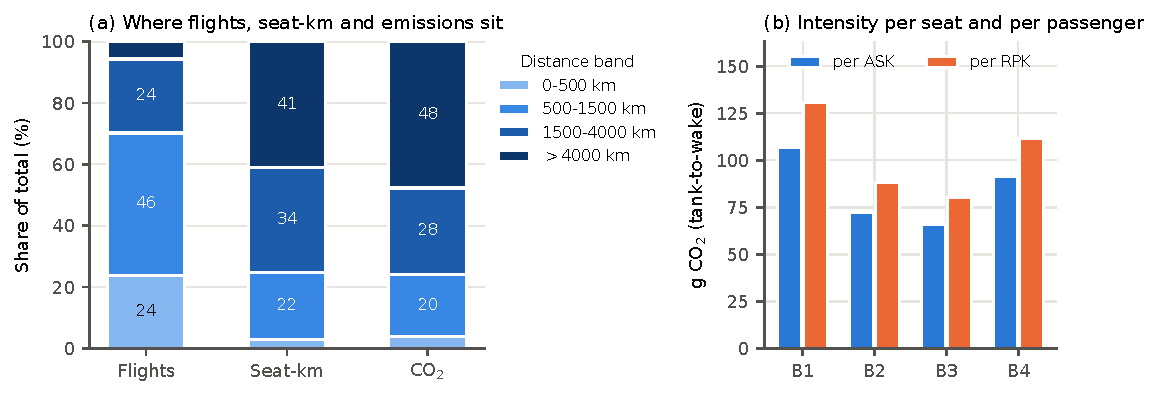
\includegraphics[width=\textwidth]{figures/fig1_band_structure}
\caption{Base-year band structure. (a) Shares of flights, seat-kilometres and
CO$_2$ by band. (b) Emissions per available seat-kilometre and per revenue
passenger-kilometre (TTW).}
\label{fig:bands}
\end{figure}

The regression of Eq.~\eqref{eq:reg} on the generated flights returns
age semi-elasticities of \GammaOne, \GammaTwo, \GammaThree\ and \GammaFour\%
per year for bands 1 to 4 (standard errors of at most \GammaSeFour\
percentage points; $H_0\!:\gamma_4=\gamma_1$ rejected, $F=\WaldF$). The
relative gradient is steeper at long range because the assumed generation step
is larger for wide-bodies than for regional aircraft
($\Delta_{\mathrm{WB}}=22\%$ against 15\%); on generated data this coefficient
reproduces an input and is reported only to show what Eq.~\eqref{eq:reg}
identifies. The robust result is the absolute one: one year of age adds about
\AbsAgeRatio\ times more CO$_2$ to a long-haul flight than to a flight below
500\,km. The load-factor coefficient is positive for emissions per flight
($\eta=\EtaFlight$) and negative for emissions per RPK ($\eta=\EtaRpk$), as
Eq.~\eqref{eq:intensity} requires.

\subsection{Pathways and attribution}
\label{sec:results-paths}

Figure~\ref{fig:paths}(a) shows the WTW emission index. Without new measures
(S0), emissions rise to an index of \IdxZero\ in 2050, as traffic growth by a
factor of \ActivityFactor\ outweighs the fleet-intensity improvement to
\PhiTwentyFifty. ATM measures (S1) lower the 2050 index to \IdxOne. The SAF
mandate (S2) reduces it to \IdxTwo, and the full portfolio (S3) to \IdxThree.
The S2 and S3 trajectories fall in steps that mirror the periods of the
mandate, most sharply in 2050.

\begin{figure}[htbp]
\centering
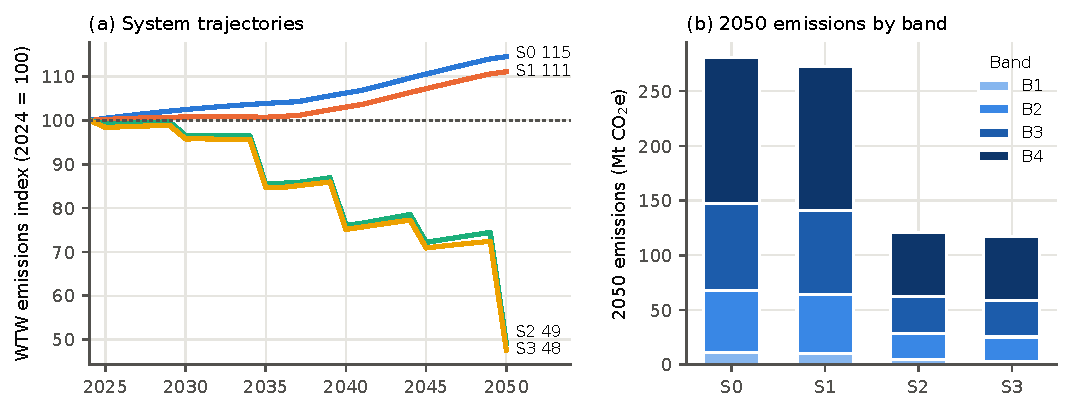
\includegraphics[width=\textwidth]{figures/fig2_trajectories}
\caption{(a) Well-to-wake emission index by pathway (2024 = 100); the steps in
S2 and S3 follow the ReFuelEU periods. (b) 2050 emissions by distance band.}
\label{fig:paths}
\end{figure}

Because scenarios activate several levers at once, differences between them do
not identify the contribution of any one lever. Figure~\ref{fig:attr} reports
the Shapley attribution of the reduction from S0 to the full lever set, by lever
and band. Of the \ShTotal\,Mt reduction in 2050, the SAF mandate contributes
\ShPctSaf\%, ATM measures \ShPctAtm\%, zero-emission propulsion \ShPctZep\% and
accelerated renewal \ShPctRenewal\%. Accelerated renewal contributes little in
2050 because natural turnover has replaced the 2024 fleet by then; its effect is
cumulative and appears in panel (b). Over 2025--2050 the shares are \ShCumPctSaf\%
for SAF, \ShCumPctAtm\% for ATM, \ShCumPctZep\% for ZEP and \ShCumPctRenewal\% for
renewal. Long-haul flights receive \ShSafLongPct\% of the SAF contribution, while
the whole ZEP contribution falls in the two shortest bands. The difference
between S3 and S2 is therefore small, and attributing it to propulsion
technology without a decomposition would overstate the role of ZEP.

\begin{figure}[htbp]
\centering
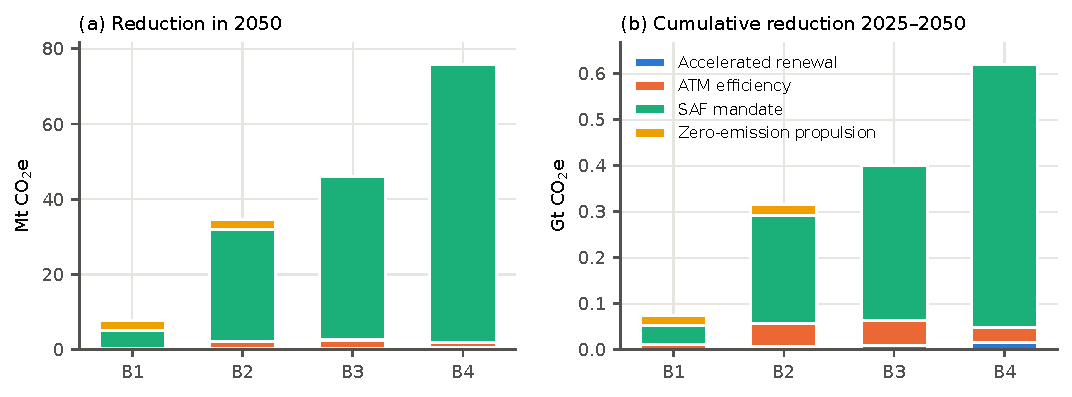
\includegraphics[width=\textwidth]{figures/fig3_attribution}
\caption{Shapley attribution of the reduction from the reference (S0) to the
full lever set, by lever and distance band. (a) 2050 emissions. (b) Cumulative
2025--2050 emissions.}
\label{fig:attr}
\end{figure}

\subsection{Tolerance to SAF supply disruption}
\label{sec:results-stress}

Figure~\ref{fig:tol} maps the cumulative excess emissions of S2 and S3 over the
$(\delta, r)$ plane. Within the range reported by \citet{martulli2025}, a
persistent 18\% shortfall ($r=0.82$) raises cumulative 2025--2050 emissions of
S2 by \CumExcessTwoRefR\%; combined with a three-year delay the excess is
\CumExcessTwoRefRDelay\%, and the 2050 level rises by \EndExcessTwoRefRDelay\%.
The two targets react very differently to delay. Because the mandate steps from
42\% to 70\% on 1 January 2050, a one-year delay raises S2's 2050 emissions by
\DelayEndTwo\% but its cumulative emissions by only \DelayCumTwo\%. A target set
on the terminal year therefore measures the timing of the last mandate step more
than the climate effect of the pathway.

\begin{figure}[htbp]
\centering
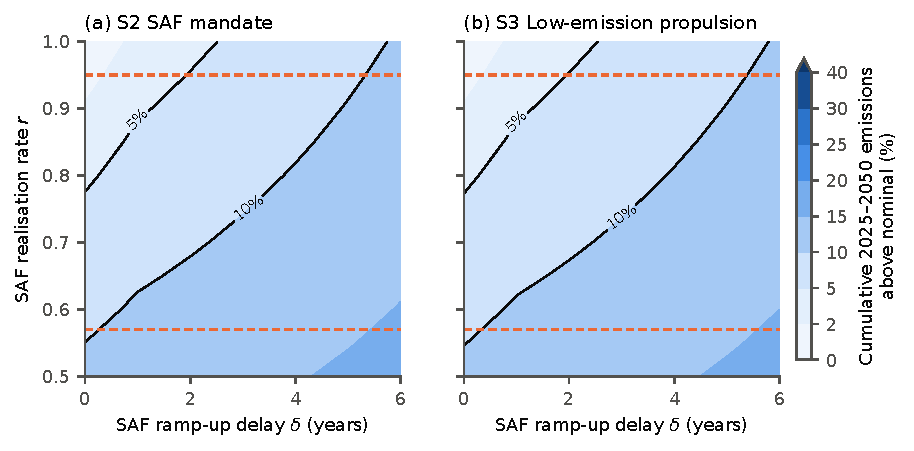
\includegraphics[width=\textwidth]{figures/fig4_tolerance}
\caption{Cumulative 2025--2050 emissions above the nominal pathway under SAF
supply disruption, by ramp-up delay $\delta$ and realisation rate $r$. Dashed
lines bound the range of realisation rates implied by \citet{martulli2025}.}
\label{fig:tol}
\end{figure}

For persistent shortfalls the critical realisation rate of Eq.~\eqref{eq:rstar}
is \RstarTwoFive, \RstarTwoTen\ and \RstarTwoTwenty\ for slacks of 5, 10 and
20\% on S2's own 2050 level, and identical to two decimals for S3. With
$\kappa_{2050}=0$ the closed form makes them exactly equal; the upstream
emissions of S3's zero-emission flights ($\kappa_{2050}=0.10$) change $r^*$ by
less than 0.01. Pathways that differ in efficiency but share the terminal blend
are therefore equally fragile against their own targets. Against an external target
common to both, set 10\% above S2's nominal 2050 level, the critical rate is
\RstarExtTwo\ for S2 and \RstarExtThree\ for S3: the additional fuel savings of
S3 buy robustness only when the target is fixed in absolute terms.

\subsection{Minimum corrective action}
\label{sec:results-corr}

Table~\ref{tab:mac} reports the static abatement cost of each corrective lever.
ATM measures have a negative net cost (\EUR{\MacAtm} per tonne CO$_2$e), because
the fuel they save is worth more than their assumed implementation cost.
Advancing the retirement of a long-haul aircraft costs \EUR{\MacRenewalLong} per
tonne and abates \AbatePerAcLong\,kt CO$_2$e per year, against
\EUR{\MacRenewalShortMin}--\MacRenewalShortMax\ per tonne and
\AbatePerAcShort--\AbatePerAcMedium\,kt per year in the other bands. Fuel savings
grow faster with distance than the capital outlay, so long-haul renewal is
cheapest per tonne as well as largest per aircraft under the stated price
assumptions. Alternative bio-SAF costs \EUR{\MacBio} and synthetic SAF
\EUR{\MacPtl} per tonne at the 2024 ReFuelEU reference prices
\citep{easa2025prices}.

\begin{table}[htbp]
\centering
\caption{Static abatement cost of corrective levers (EUR per t CO$_2$e, WTW,
2030) and annual abatement per early-retired aircraft.}
\label{tab:mac}
\small
\begin{tabular}{lrr}
\toprule
Lever & EUR/t CO$_2$e & kt CO$_2$e per aircraft-year \\
\midrule
\csname @@input\endcsname generated/tab_mac.tex
\bottomrule
\end{tabular}
\end{table}

Table~\ref{tab:corr} and Figure~\ref{fig:corr} report the solutions of
programme~\eqref{eq:lp} for four reference disruptions, first with only the
cumulative budget as target and then with both targets. For S2 under an 18\%
shortfall without delay, the cumulative gap is \CorrNoDelayGap\,Mt CO$_2$e.
Restoring the budget alone requires ATM measures and the early retirement of
\CorrNoDelayCumLong\ long-haul aircraft and yields a net saving of
\EUR{\CorrNoDelayCumSaving}\,bn, because under the assumed fuel and aircraft
prices both levers save more fuel than they cost. Restoring the 2050 level as
well raises the cost to \EUR{\CorrNoDelayCost}\,bn: the 2050 constraint can only
be met by actions that save fuel in 2050 itself, which requires renewal in the
other bands and alternative SAF, and \CorrNoDelayResEnd\% of the 2050 gap still
remains. Restricted to a single lever, ATM measures close only
\SingleATMCovered\% of the cumulative gap, whereas renewal alone or alternative
SAF alone can close it. Under a three-year delay with the same shortfall, the
cumulative gap grows to \CorrDelayGap\,Mt and costs \EUR{\CorrDelayCumCost}\,bn
to close (\EUR{\CorrDelayCost}\,bn with both targets), and \CorrDelayResEnd\% of
the 2050 gap cannot be closed within the delivery-slot and supply limits.

\begin{table}[htbp]
\centering
\caption{Minimum-cost corrective portfolios. Gaps in Mt CO$_2$e (cumulative
2025--2050 and in 2050). Lever quantities refer to the programme with both
targets: ATM in Mt fuel saved; aircraft retired early (cumulative); alternative
SAF in Mt. Net cost in bn EUR when only the cumulative budget is restored and
when both targets are pursued; negative values are net savings. Residuals are
the uncompensated shares of the cumulative and 2050 gaps (\%). Disruption given
as $(\delta, r)$.}
\label{tab:corr}
\small
\footnotesize
\setlength{\tabcolsep}{2.5pt}
\begin{tabular}{llrrrrrrrrrr}
\toprule
 & & \multicolumn{2}{c}{Gap} & ATM & \multicolumn{2}{c}{Early retirement} & Alt. & \multicolumn{2}{c}{Cost} & \multicolumn{2}{c}{Residual} \\
\cmidrule(lr){3-4}\cmidrule(lr){6-7}\cmidrule(lr){9-10}\cmidrule(lr){11-12}
Path & $(\delta, r)$ & cum. & 2050 & fuel & $>$4000\,km & other & SAF & cum. & both & cum. & 2050 \\
\midrule
\csname @@input\endcsname generated/tab_corrective.tex
\bottomrule
\end{tabular}
\end{table}

\begin{figure}[htbp]
\centering
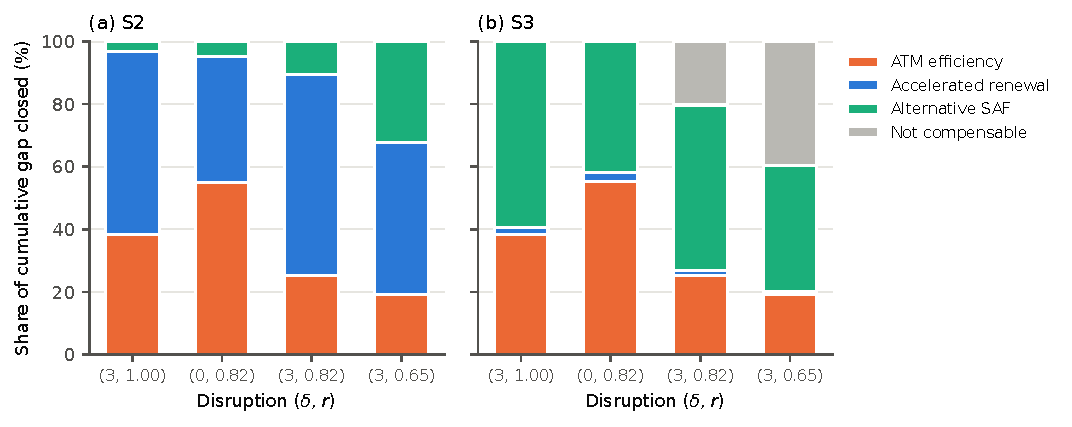
\includegraphics[width=\textwidth]{figures/fig5_corrective}
\caption{Composition of the minimum-cost corrective portfolio (both targets) as
a share of the cumulative 2025--2050 gap. Grey: part of the cumulative gap that
cannot be closed within the lever limits.}
\label{fig:corr}
\end{figure}

S3 is less correctable than S2. Its own accelerated renewal already uses almost
all delivery slots, so the renewal lever is nearly exhausted when a disruption
occurs. The corrective programme must then rely on alternative SAF, which is
more expensive: restoring the cumulative budget after an 18\% shortfall costs
\EUR{\CorrThreeNoDelayCumCost}\,bn, and \CorrThreeNoDelayResEnd\% of the 2050 gap
remains open even without delay. When a three-year delay is combined with a
shortfall of 18\% or more, up to \ResCumThreeMax\% of the cumulative gap also
remains uncompensated. A pathway that pre-commits a scarce resource to its nominal plan
has less of it left as a reserve.

\subsection{Sensitivity}

Figure~\ref{fig:sens} varies eight parameters one at a time for S2 under an 18\%
shortfall with both targets. To keep outcomes comparable, any residual the
levers cannot close, cumulative or in 2050, is priced at the synthetic-SAF
abatement cost. The resulting corrective cost of \EUR{\SensRef}\,bn is most
sensitive to the implementation cost of ATM measures
and to the fossil fuel price, both of which determine the net cost of fuel
savings; the widest range is \EUR{\SensMaxSpread}\,bn. The life-cycle reduction
of bio-SAF barely matters, because it scales the gap and the abatement of
alternative SAF alike. Long-haul renewal remains the cheapest renewal option in
every variation. ATM measures remain cheaper than long-haul renewal as long as
their gross implementation cost stays below about \EUR{\AtmBreakeven} per tonne
of CO$_2$; at the high value of the range the two swap places.

\begin{figure}[htbp]
\centering
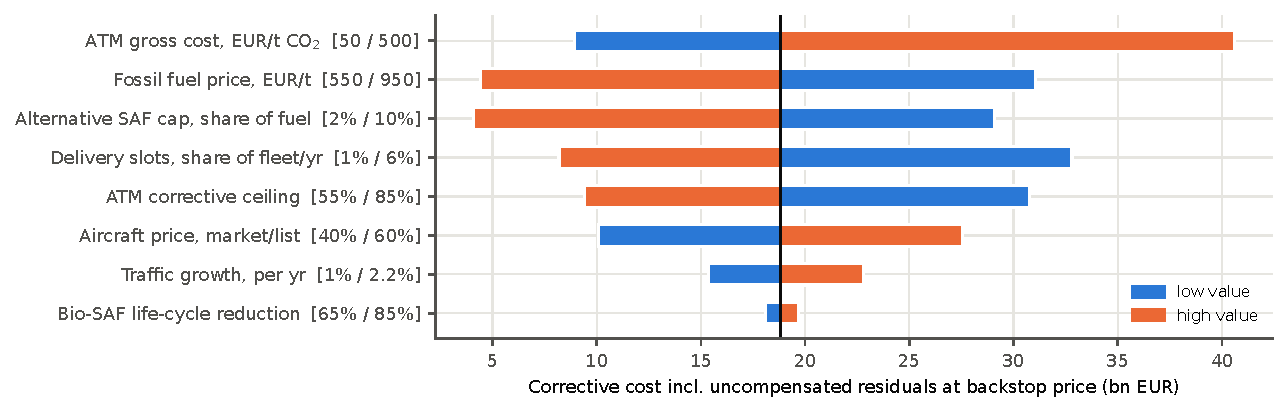
\includegraphics[width=\textwidth]{figures/fig6_sensitivity}
\caption{One-at-a-time sensitivity of the corrective cost (both targets) for S2
under an 18\% shortfall without delay, with uncompensated residuals priced at
the synthetic-SAF abatement cost. Low and high values in brackets.}
\label{fig:sens}
\end{figure}

%% ===========================================================================
\section{Economic, management and policy implications}
\label{sec:discussion}

\subsection{ATM as the first buffer against SAF shortfalls}

ATM measures have a negative net cost under the stated assumptions, and their
benefit is concentrated in the short- and medium-haul bands where fleet renewal has the
least leverage. They are, however, small: even at a recovery ceiling of 70\% of
the benefit pool, they close only about half of the cumulative gap from an 18\%
shortfall. The model lets every lever act from 2025; in practice ATM measures
can also be deployed faster than fleet renewal, which is constrained by
manufacturing lead times, so the model understates their value as a near-term
buffer. Two implications follow for performance regulation under the Single
European Sky. First, environmental targets for air navigation service providers
can be framed as a contingency instrument: the benefit pool not yet recovered is
a reserve that can be mobilised when fuel supply falls short. Second, because
the pool is largest in relative terms on short flights, terminal-area measures
(taxi and arrival management) deserve weight comparable to en-route flight
efficiency, which dominates the current indicators.

\subsection{SAF target design}

The stepwise mandate makes the 2050 level hostage to the timing of the last
step. A one-year slip changes 2050 emissions by about half but cumulative
emissions by a few percent. Monitoring progress against a cumulative budget, or
against interim milestones between the five-year steps, would align the
assessment with the physical climate effect and reduce the incentive to judge
pathways by a single year. For fuel suppliers and airlines, the results quantify
the value of contingency arrangements, such as import options and book-and-claim
supply, that can be activated when domestic capacity is late.

\subsection{Fleet planning and corrective headroom}

Per aircraft and per euro, advancing the retirement of long-haul aircraft is
the most effective renewal measure, so fleet-renewal support aimed at emissions
should not be distributed evenly across the network. Delivery slots, however,
are scarce. A pathway that commits them in advance to accelerated renewal
reduces its emissions but loses the ability to respond when SAF falls short.
For airlines and policymakers this is a portfolio question: part of the renewal
capacity has option value as a reserve, and committing it fully trades
robustness for expected reductions.

\subsection{Who bears the corrective cost}

The levers belong to different actors. ATM measures are delivered by air
navigation service providers and the Network Manager under performance
regulation; early retirement is an airline decision constrained by manufacturers'
backlogs; alternative SAF is procured by fuel suppliers, whose shortfalls are
penalised with reference to the published prices. The corrective portfolios in
Table~\ref{tab:corr} therefore require coordination. In S2 the least-cost
response to a supply shortfall lies mostly with air navigation service providers
and airlines rather than with the fuel suppliers who bear the mandate. In S3,
where renewal capacity is already committed, alternative SAF procured by fuel
suppliers closes \AltShareThreeMin--\AltShareThreeMax\% of the cumulative gap.

\subsection{Limitations}

Four limitations qualify the results. First, the base-year flight population is
generated rather than observed. It reproduces the published band shares and
passes independent checks, but the within-band regressions on generated data
reproduce their inputs and are not evidence; the pipeline accepts observed
flights with the same schema, and replication on such data is the most important
extension. Second, the model is restricted to CO$_2$ on a WTW basis. Non-CO$_2$
effects, contrails in particular, are of similar magnitude
\citep{lee2021}, are distance- and altitude-dependent, and would change both the
allocation question of Eq.~\eqref{eq:neutral} and the value of ATM measures,
which can be used to avoid contrail formation. Third, costs are static and
undiscounted over the corrective window, demand does not respond to cost
pass-through, and the corrective programme abstracts from aircraft reassignment
across markets. Fourth, the stress test is a deterministic grid; attaching
probabilities to $(\delta, r)$, for example from the diffusion scenarios of
\citet{martulli2025}, would convert the tolerance maps into probabilities of
meeting each target. The geographic scopes also differ: the inventory covers the
EUROCONTROL area, whereas ReFuelEU applies at Union airports.

%% ===========================================================================
\section{Conclusions}
\label{sec:conclusions}

This paper developed a well-to-wake, distance-band model of European aviation
emissions and used it to ask how much SAF supply shortfall decarbonisation
pathways can absorb and how it can be compensated at least cost. Four results
stand out. First, emissions concentrate in long-haul flying while ATM
inefficiency concentrates in short-haul flying, so the levers that can act
quickly and those that act where emissions are largest belong to different
bands. Second, the SAF mandate delivers most of the reduction of the full
portfolio, and the step structure of the mandate makes terminal-year targets far more
sensitive to supply timing than cumulative budgets. Third, after a supply
shortfall the cumulative budget can be restored mainly through ATM measures and
early retirement of long-haul aircraft, at low or negative net cost under the
assumed prices; restoring the 2050 level as well is considerably more expensive,
and under multi-year delays most of the 2050 gap cannot be closed within
manufacturing and supply limits.
Fourth, pathways that commit scarce delivery slots in advance retain the least
corrective headroom.

For policy, the results support assessing ReFuelEU progress against cumulative
budgets or interim milestones, treating the unrecovered ATM benefit pool as a
contingency reserve, and directing fleet-renewal support to long-haul aircraft
while preserving part of the renewal capacity as an option. Future work should
replicate the analysis on observed flight-level data, add non-CO$_2$ effects,
and attach probabilities to the disruption space.

%% ===========================================================================
\section*{Data and code availability}
The model, parameter file with sources, and the script that reproduces every
number, table and figure in this paper are available in a public repository
\ifanon [link withheld for review]\else [repository URL]\fi.

\section*{Declaration of generative AI use}
% AUTHORS: complete according to the journal's policy.

\section*{CRediT authorship contribution statement}
% AUTHORS: complete.

\section*{Declaration of competing interest}
The authors declare that they have no known competing financial interests or
personal relationships that could have appeared to influence the work reported
in this paper.

\appendix
\section{Parameters and sources}
\label{app:params}

\scriptsize
\setlength{\tabcolsep}{3pt}
\begin{longtable}{>{\raggedright\arraybackslash}p{0.27\textwidth}>{\raggedright\arraybackslash}p{0.17\textwidth}>{\raggedright\arraybackslash}p{0.11\textwidth}>{\raggedright\arraybackslash}p{0.37\textwidth}}
\toprule
Parameter & Value & Status & Source or rationale \\
\midrule
\endhead
\csname @@input\endcsname generated/tab_parameters.tex
\bottomrule
\end{longtable}
\normalsize

\bibliographystyle{elsarticle-harv}
\bibliography{refs}

\end{document}
